%%%%%%%%%%%%%%%%%%%%%%%%%%%%%%%%%%%%%%%%%%%%%%%%%%%%%%%%%%
%
% Vzor pro sazbu kvalifikační práce
%
% Západočeská univerzita v Plzni
% Fakulta aplikovaných věd
% Katedra informatiky a výpočetní techniky
%
% Petr Lobaz, lobaz@kiv.zcu.cz, 2016/03/14
%
%%%%%%%%%%%%%%%%%%%%%%%%%%%%%%%%%%%%%%%%%%%%%%%%%%%%%%%%%%

% Možné jazyky práce: czech, english
% Možné typy práce: BP (bakalářská), DP (diplomová)
\documentclass[czech,DP]{thesiskiv}

% Definujte údaje pro vstupní strany
%
% Jméno a příjmení; kvůli textu prohlášení určete, 
% zda jde o mužské, nebo ženské jméno.
\author{Bc. Vojtěch Danišík}
\declarationmale

% Název práce
\title{Tvorba rozsáhlých úložišť patentových dat}

% 
% Texty abstraktů (anglicky, česky)
%
\abstracttexten{Creation of large-scale patent data repositories. The aim of the diploma thesis is to get acquainted with the available sources of patent data and to create extensive local repositories of patent data enabling their effective searching and mining. The first part of the thesis thoroughly describes the types of patents, existing data sources and file formats in which patents are stored. Subsequently, the applicable technologies for searching and mining are described. The second part of the thesis is devoted to the selection of usable data and the implementation of selected technologies. Several queries and scenarios have been created to test efficient mining. The results of the testing are part of this work.
}

\abstracttextcz{Cílem diplomové práce je seznámit se s dostupnými zdroji dat o patentech a vytvořit rozsáhlá lokální úložiště patentových dat umožňující jejich efektivní prohledávání a vytěžování. První část práce důkladně popisuje typy patentů, existující zdroje dat a formáty souborů, ve kterých se patenty ukládají. Následně jsou popsány použitelné technologie pro prohledávání a vytěžování. Druhá část práce se věnuje výběru použitelných dat a implementaci vybraných technologií. Pro otestování efektivního vytěžování  bylo vytvořeno několik dotazů a scénářů. Výsledky testování jsou součástí této práce.
}

% Na titulní stranu a do textu prohlášení se automaticky vkládá 
% aktuální rok, resp. datum. Můžete je změnit:
%\titlepageyear{2016}
%\declarationdate{1. března 2016}

% Ve zvláštních případech je možné ovlivnit i ostatní texty:
%
%\university{Západočeská univerzita v Plzni}
%\faculty{Fakulta aplikovaných věd}
%\department{Katedra informatiky a výpočetní techniky}
%\subject{Bakalářská práce}
%\titlepagetown{Plzeň}
%\declarationtown{Plzni}

%%%%%%%%%%%%%%%%%%%%%%%%%%%%%%%%%%%%%%%%%%%%%%%%%%%%%%%%%%
%
% DODATEČNÉ BALÍČKY PRO SAZBU
% Jejich užívání či neužívání záleží na libovůli autora 
% práce
%
%%%%%%%%%%%%%%%%%%%%%%%%%%%%%%%%%%%%%%%%%%%%%%%%%%%%%%%%%%

% Zařadit literaturu do obsahu
\usepackage[nottoc,notlot,notlof]{tocbibind}

% Umožňuje vkládání obrázků
\usepackage[pdftex]{graphicx}

% Odkazy v PDF jsou aktivní; navíc se automaticky vkládá
% balíček 'url', který umožňuje např. dělení slov
% uvnitř URL
\usepackage[pdftex]{hyperref}
\hypersetup{colorlinks=true,
  unicode=true,
  linkcolor=black,
  citecolor=black,
  urlcolor=black,
  bookmarksopen=true}

% Při používání citačního stylu csplainnatkiv
% (odvozen z csplainnat, http://repo.or.cz/w/csplainnat.git)
% lze snadno modifikovat vzhled citací v textu
\usepackage[numbers,sort&compress]{natbib}
\usepackage[dvipsnames]{xcolor}
\usepackage{array}
\usepackage{float}
\usepackage{textcomp}
\usepackage[colorinlistoftodos,prependcaption,textsize=tiny]{todonotes}
\usepackage{listings,xcolor}
\usepackage{verbatim}
\usepackage{fancyhdr}

% Acronyms
\usepackage[nomain, abbreviations, automake]{glossaries-extra}
\makeglossaries
\setabbreviationstyle{long-short}
\setabbreviationstyle[acronym]{short}
% Databáze
\newacronym{DBMS}{DBMS}{Database Management Systems}
\newacronym{ACID}{ACID}{Atomicity, Consistency, Isolation, Durability}
\newacronym{JSON}{JSON}{JavaScript Object Notation}
\newacronym{SQL}{SQL}{Structured Query Language}
\newacronym{XML}{XML}{Extensible Markup Language}
\newacronym{BSON}{BSON}{Binary JSON}

% Návrh uložiště
\newacronym{EPO}{EPO}{European Patent Office}
\newacronym{WIPO}{WIPO}{World Intellectual Property Organization}
\newacronym{USPTO}{USPTO}{United States Patent and Trademark Office}


% Rozšiřitelnost
\newacronym{CSV}{CSV}{Comma-separated values}
\newacronym{URL}{URL}{Uniform Resource Locator}

\lstdefinestyle{sqlstyle}{
language = sql,
frame = single,
basicstyle = \small\ttfamily,
breaklines = true,
showtabs = false,
showstringspaces = false,
stringstyle = \color{red},
identifierstyle = \color{blue},
commentstyle = \color{gray},
numberstyle = \color{yellow},
emph =[1]{inventors, ., patents, applicants, classification},
emphstyle =[1]\color{black}\bfseries,
}

%%%%%%%%%%%%%%%%%%%%%%%%%%%%%%%%%%%%%%%%%%%%%%%%%%%%%%%%%%
%
% VLASTNÍ TEXT PRÁCE
%
%%%%%%%%%%%%%%%%%%%%%%%%%%%%%%%%%%%%%%%%%%%%%%%%%%%%%%%%%%
\begin{document}
%
\maketitle
\pagestyle{empty}
\tableofcontents
\pagestyle{plain}
\addtocontents{toc}{
\protect\thispagestyle{empty}} 

\thispagestyle{empty}
\setcounter{page}{0} 

%CHAPTER
\chapter{Úvod}
Patenty jsou v dnešní době nedílnou součástí zákonné ochrany nových technologií a vynálezů v průmyslu a jejich odvětví. Vlastník takového patentu má výhradní právo využívat vynález a poskytovat souhlas o využití patentu jiným stranám. Patenty jsou registrovány a spravovány jak v rámci jednotlivých zemí (národní patentové instituce), tak i mezinárodně (například Evropský patentový úřad \gls{EPO}). Tyto instituce veřejně poskytují informace o registrovaných patentech pomocí vyhledávačů na jejich webových stránkách. Pro vědce a vynálezce jsou tyto vyhledávače velice důležité právě proto, aby si mohli zkontrolovat, zda jejich vynález je jedinečný, nebo už ve světe existuje v lehce upravené podobě a je patentován.
\newline
\indent Cílem této práce je se seznámit s dostupnými zdroji dat o patentech a vytvořit rozsáhlá lokální úložiště patentových dat umožňující jejich efektivní vytěžování. Zdroje dat musí poskytovat své databáze patentů (žádosti i publikace) zdarma a patenty musí obsahovat předem stanovené povinné atributy, aby je bylo možné použít. Získaná data budou následně uložena do specifického typu databáze, která bude umožňovat co nejefektivnější vytěžování uložených dat. To znamená rychlé vyhledávání správných výsledků v relativně krátkém čase pro miliony (až desítky milionů) záznamů. Stažená data budou filtrována na základě specifikovaných atributů, které musí obsahovat (protože ve struktuře existuje element pro povinný atribut ještě neznamená, že pro něj existuje reálná hodnota).
%CHAPTER
\chapter{Patent}
\todo{todo}
základní informace + uložiště dat + info o zdrojích (patentové úřady atp) \newline
\section{Patent vs Užitný vzor}
\section{Patent vs Průmyslový vzor}
\section{Patent vs Ochranná známka}
\section{Patent vs Autorská práva}


%%%%%%%%%%%%%%%%%%%%%%%%%%%%%%%%%%%%%%%%%%%%%%%%%%%%%%%%%%%%

%CHAPTER
\chapter{Databáze}

Termín databáze označuje organizovanou kolekci strukturovaných informací nebo dat, která jsou typicky ukládána elektronicky v počítačovém systému. Data / informace lze nazvat jako fakta vztahující se k libovolnému uvažovanému objektu. Typický příklad objektu je člověk, jehož fakta jsou: jméno, věk, výška, váha a mnoho dalších \cite{guru99Database}.\newline

\section{Systém řízení báze dat}
Pro správu dat v databázi a její řízení je potřeba komplexní software, který se nazývá \textbf{Systém Řízení Báze Dat} (SŘBD, anglicky \gls{DBMS}). SŘBD slouží jako interface mezi samotnou databází a koncovým uživatelem (může být i program), umožňující jak vytěžování a aktualizaci dat, tak i možnosti nastavení záloh a jiných administrativních operací \cite{OracleDB}. V dnešním světe existuje několik různých \gls{DBMS} (například Relační \gls{DBMS}, Objektově-orientované \gls{DBMS}).
\begin{figure}[h!]
\centering
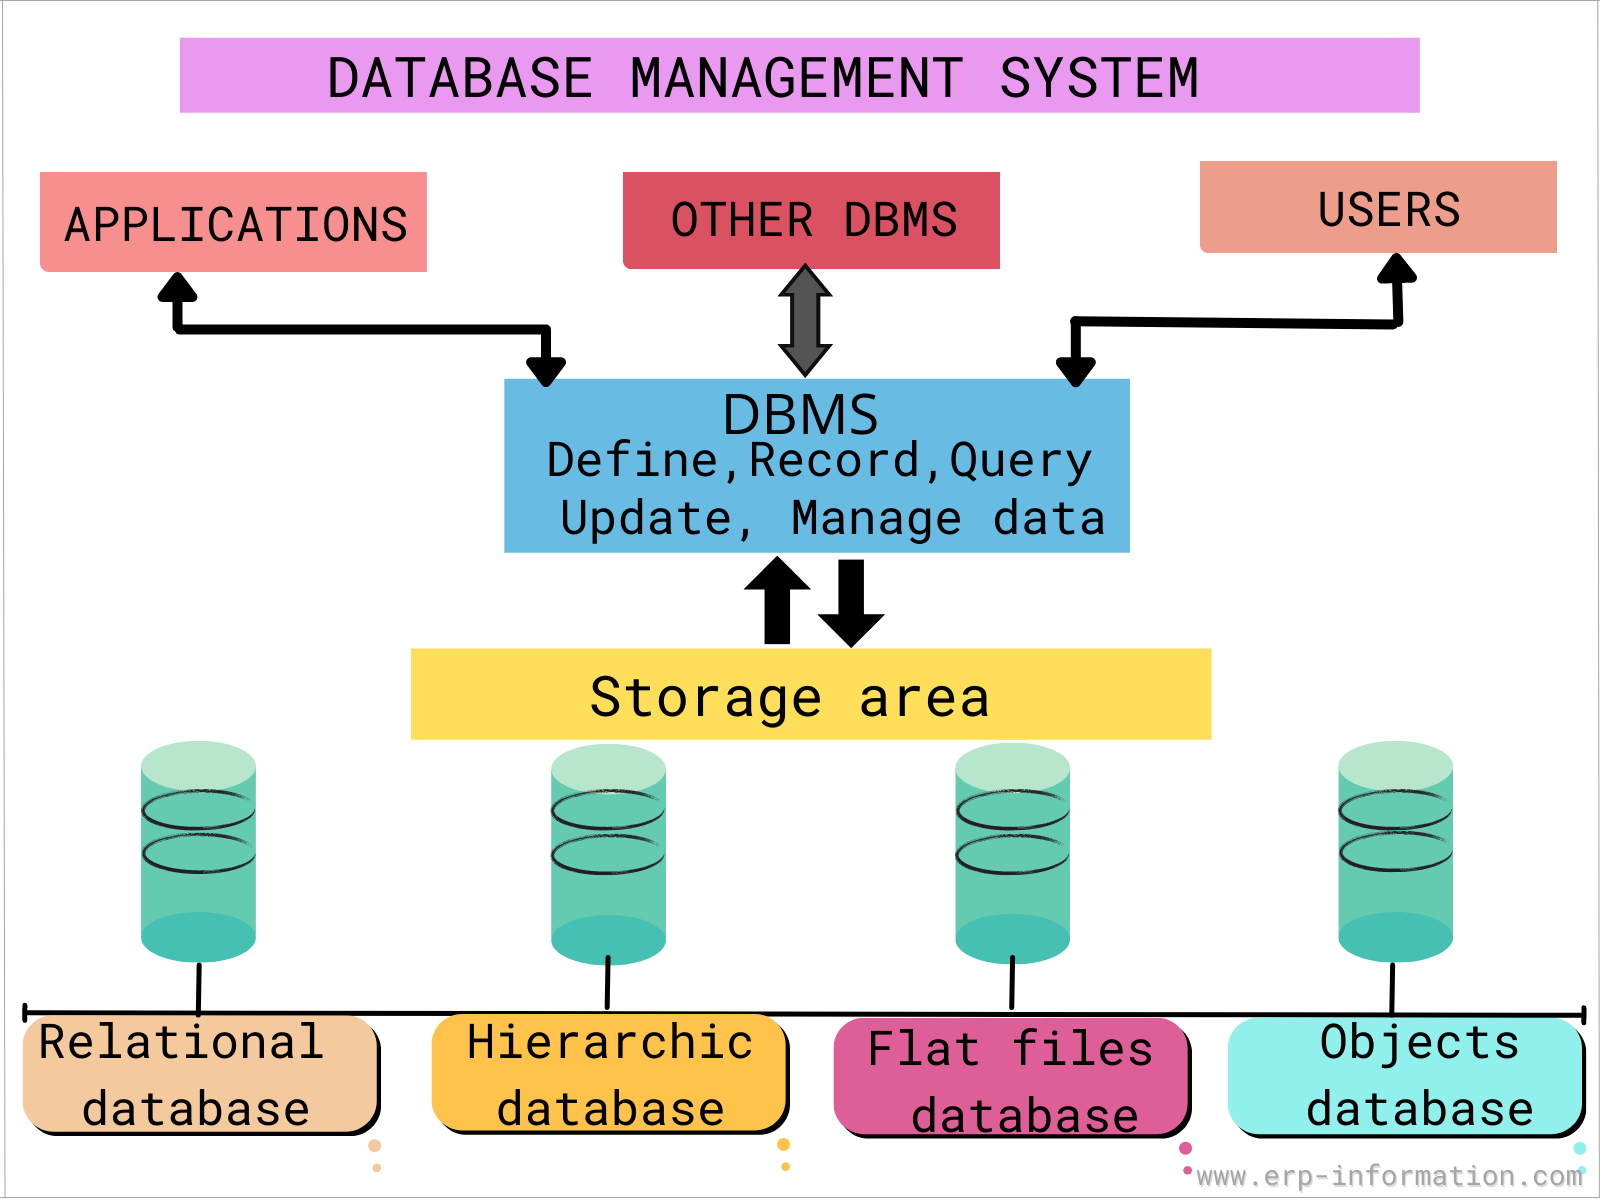
\includegraphics[width=10cm]{img/databaze/dbms}
\caption{Systém řízení báze dat}
\label{fig:dbms}
\end{figure}

\section{Komponenty databáze}
Všechny databáze sestávají z pěti základních komponent, nehledě na použitý typ databáze \cite{TechTargetDB, guru99Database}:
\begin{itemize}
\item \textbf{Hardware} - Fyzické stroje (počítače, servery, pevné disky, ...) na kterých běží databázový software.
\item \textbf{Software} - Databázový software poskytuje uživateli / programu kontrolu nad databází. Zahrnuje to samotný databázový software, operační systém, software pro správu sdílení dat mezi uživately a programy pro přístup k datům v databázi.
\item \textbf{Data} - Nezpracované a neorganizované fakty, které je potřeba zpracovat. Administrátor databáze organizuje tyto data a dává jim význam. Data se obecně skládají hlavně z faktů, observací, percepcí, čísel, znaků a mnoho dalších.
\item \textbf{Jazyk} - Typický příklad použití jazyku je přístup k datům, přidávání nových dat, úpravu již existujících dat z databáze. Uživatel / program napíše specifické příkazy v jazyku pro přístup k datům (Database Access Language) a tyto příkazy následně pošle databázi ke zpracování. Více viz kapitola č. \ref{sec:jazyky}.
\item \textbf{Procedury} - Procedura obsahuje předpřipravený seznam příkazů, které se následně vykonávají po zavolání dané procedury. 
\end{itemize}

\section{Jazyky} \label{sec:jazyky}
Databázové jazyky, jinak známé jako dotazovací jazyky, jsou klasifikací programovacích jazyků, které se používají k definování a přístupu k databázím. Pomocí těchto jazyků dokáže uživatel získávat nebo spravovat data v databázích. V dnešní době se jazyky (například \gls{SQL}) mohou skládat ze čtyř podjazyků, kdy každý slouží k jinému účelu v rámci vykonávání příkazů \cite{indeedDBLanguage, begginersBookDBLanguage}:
\begin{itemize}
\item \textbf{Data definition language} (DDL) - DDL umí vytvářet jednotlivé komponenty databázového schématu (tabulky, soubory, indexy, ...), které tvoří strukturu reprezentující organizaci dat v databázi. Dostupné příkazy pro jazyk DDL:
	\begin{itemize}
	\item \textbf{CREATE} - Vytvoření nového objektu (tabulka, index, ...).
	\item \textbf{ALTER} - Změna struktury objektu.
	\item \textbf{DROP} - Smazání objektu.
	\item \textbf{RENAME} - Změna názvu objektu.
	\item \textbf{TRUNCATE} - Smazání podobjektů v objektu (například záznamy v tabulce).
	\end{itemize}
\item \textbf{Data manipulation language} (DML) - DML slouží pro manipulaci s daty, které se nachází v již existující databázi. Dostupné příkazy pro jazyk DML:
	\begin{itemize}
	\item \textbf{SELECT} - Získání záznamů (dat) z tabulky.
	\item \textbf{INSERT} - Vložení nového záznamu (dat) do tabulky.
	\item \textbf{UPDATE} - Úprava existujícího záznamu v tabulce.
	\item \textbf{DELETE} - Smazání záznamu z tabulky.
	\end{itemize}
\item \textbf{Data control language} (DCL) - Pomocí DCL lze kontrolovat přístupy a práva k datům, které jsou uloženy v databázi. Uživateli lze nastavit práva k jednotlivým DML příkazům nad tabulkama / procedurama (například uživatel bude mít přístup pouze k příkazu SELECT nad tabulkou "TABULKA"). Dostupné příkazy pro jazyk DCL:
	\begin{itemize}
	\item \textbf{GRANT} - Přidání práv uživateli nad danou tabulkou / procedurou. 
	\item \textbf{REVOKE} - Odebrání práv uživateli nad danou tabulkou / procedurou.
	\end{itemize}

\item \textbf{Transaction control language} (TCL) - TCL spravuje transakce v databázi. Transakce obsahuje jeden či více DML příkazů nad tabulkama, které se vykonávají po sobě. Všechny příkazy musí být úspěšně provedeny, aby bylo možné transakci označit za úspěšnou. Ukázka jedné transakce viz obrázek č. \ref{fig:tcl_savepoint}. Dostupné příkazy pro jazyk TCL:
	\begin{itemize}
	\item \textbf{COMMIT} - Potvrzení transakce, změny provedené v transakci jsou permanentní a nejdou vzít zpět.
	\item \textbf{ROLLBACK} - Vezme zpět veškerou práci v aktuální transakci. Lze se vrátit na začátek transakce nebo k SAVEPOINTu.
	\item \textbf{SAVEPOINT} - Nastavení bodu v transakci, ke kterému se lze v budoucnu vrátit pomocí ROLLBACK.
	\end{itemize}
\end{itemize}
	\begin{figure}[H]
	\centering
	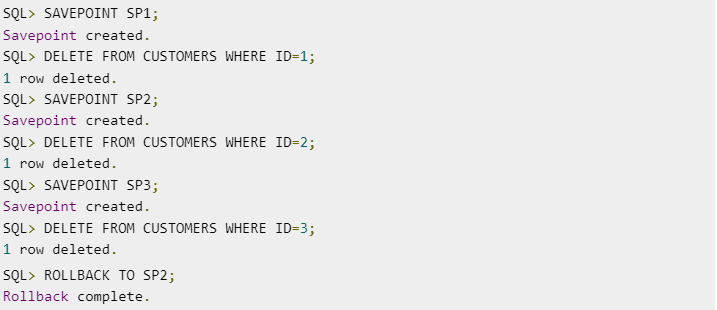
\includegraphics[width=14cm]{img/databaze/tcl_savepoint}
	\caption{Ukázka jedné transakce (bez commitu)}
	\label{fig:tcl_savepoint}
	\end{figure}
\section{Typy databází}
V dnešním světě existuje mnoho různých typů databází. Výběr nejlepšího typu databáze pro konkrétní organizaci závisí na tom, jak organizace zamýšlí data používat. V této kapitole je vypsáno pouze pár typů, protože vznikají stále nové, méně známé typy databází, které jsou tvořeny pro specifické požadavky (například finanční, věděcké) \cite{matillionTypeDB, OracleDB}.
\subsection{Relační databáze}
Název relační databáze pochází ze způsobu, jakým jsou data uložena, a to ve více souvisejících tabulkách. Data v tabulkách jsou uložena v řádcích a sloupcích. Relační databáze jsou velice spolehlivé a podporují všechny čtyři žádoucí vlastnosti databázových transakcí \gls{ACID}. Pro co nejefektivěnjší využití tohoto typu databáze je potřeba ukládat pouze dobře strukturovaná data, pro částečně strukturovaná či nestrukturovaná data je vhodné použít například grafové nebo dokumentově založené databáze. Typické relační databáze jsou například: Microsoft SQL Server, Oracle Database, MySQL, PostgreSQL. Ukázku relační databáze lze vidět na obrázku č. \ref{fig:db_img_relational}.
	\begin{figure}[H]
	\centering
	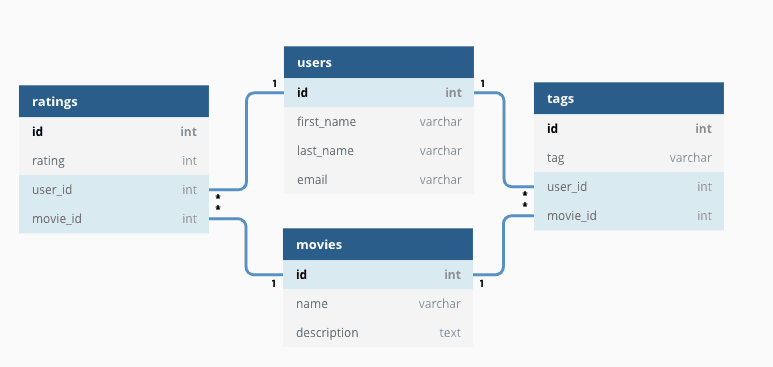
\includegraphics[width=14cm]{img/databaze/relational_db}
	\caption{Ukázka relační databáze}
	\label{fig:db_img_relational}
	\end{figure}
\subsection{Objektově-orientovaná databáze}
Objektově-orientovaná databáze je založena na objektově-orientovaném programování, kdy data a všechny jejich atributy a metody jsou svázány dohromady jako objekt. Stejně jako relační databáze, i objektově-orientované databáze odpovídají standardům \gls{ACID}. Typické příklady jsou například: ObjectStore, ConceptBase. Ukázku objektově-orientované databáze lze vidět na obrázku č. \ref{fig:db_img_oo}.
	\begin{figure}[H]
	\centering
	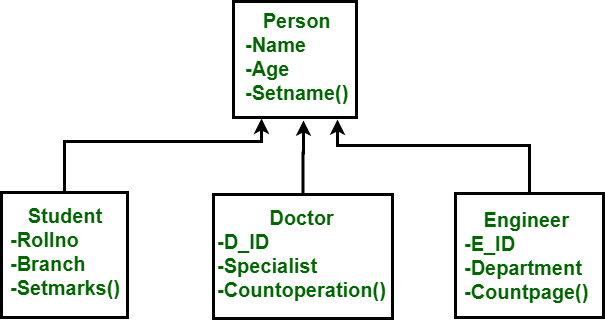
\includegraphics[width=12cm]{img/databaze/oo_db}
	\caption{Ukázka objektově-orientované databáze}
	\label{fig:db_img_oo}
	\end{figure}
\subsection{NoSQL databáze}
NoSQL je široká kategorie databází, které nepoužívají \gls{SQL} jako svůj primární jazyk pro přístup k datům. Tyto typy databází jsou také někdy označovány jako nerelační databáze. V NoSQL databázích se pracuje s nestrukturovanými a polostrukturovanými sadami distribuovaných dat. Jednou z výhod je, že vývojáři mohou provádět změny databáze za běhu, aniž by to ovlivnilo aplikace, které databázi používají.
\subsection{Databáze Klíč-Hodnota}
Databáze klíč-hodnota poskytuje nejjednodušší možný NoSQL datový model. Data jsou uložená jako pár klíč - hodnota ve slovníku / mapě, kdy klíč je indexem. Hodnota může být například celé číslo, řetězec, struktura \gls{JSON} nebo pole. Typické příklady jsou: Redis, Riak, LevelDB. Ukázku databáze klíč-hodnota lze vidět na obrázku č. \ref{fig:db_img_keyvalue}.
	\begin{figure}[H]
	\centering
	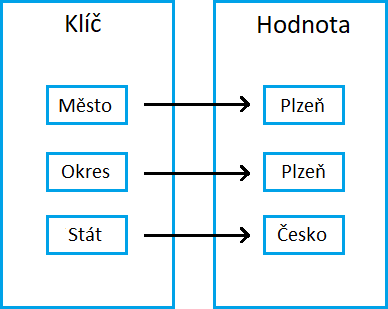
\includegraphics[width=10cm]{img/databaze/keyvalue_db}
	\caption{Ukázka databáze klíč-hodnota.}
	\label{fig:db_img_keyvalue}
	\end{figure}
\subsection{Grafová databáze}
Grafová databáze je typem NoSQL databáze, která je založená na teorii grafů. Data jsou reprezentována jako uzly, hrany zase reprezentují vztahy mezi daty. Graf lze procházet podél určitých typů hran nebo přes celý graf. Procházení spojení nebo relací je velmi rychlé, protože vztahy mezi uzly se nepočítají v době dotazu, ale jsou v databázi trvalé. Typické příklady jsou: Neo4j, OrientDB, Microsoft Azure CosmosDB. Ukázku grafové databáze lze vidět na obrázku č. \ref{fig:db_img_graph}.
	\begin{figure}[H]
	\centering
	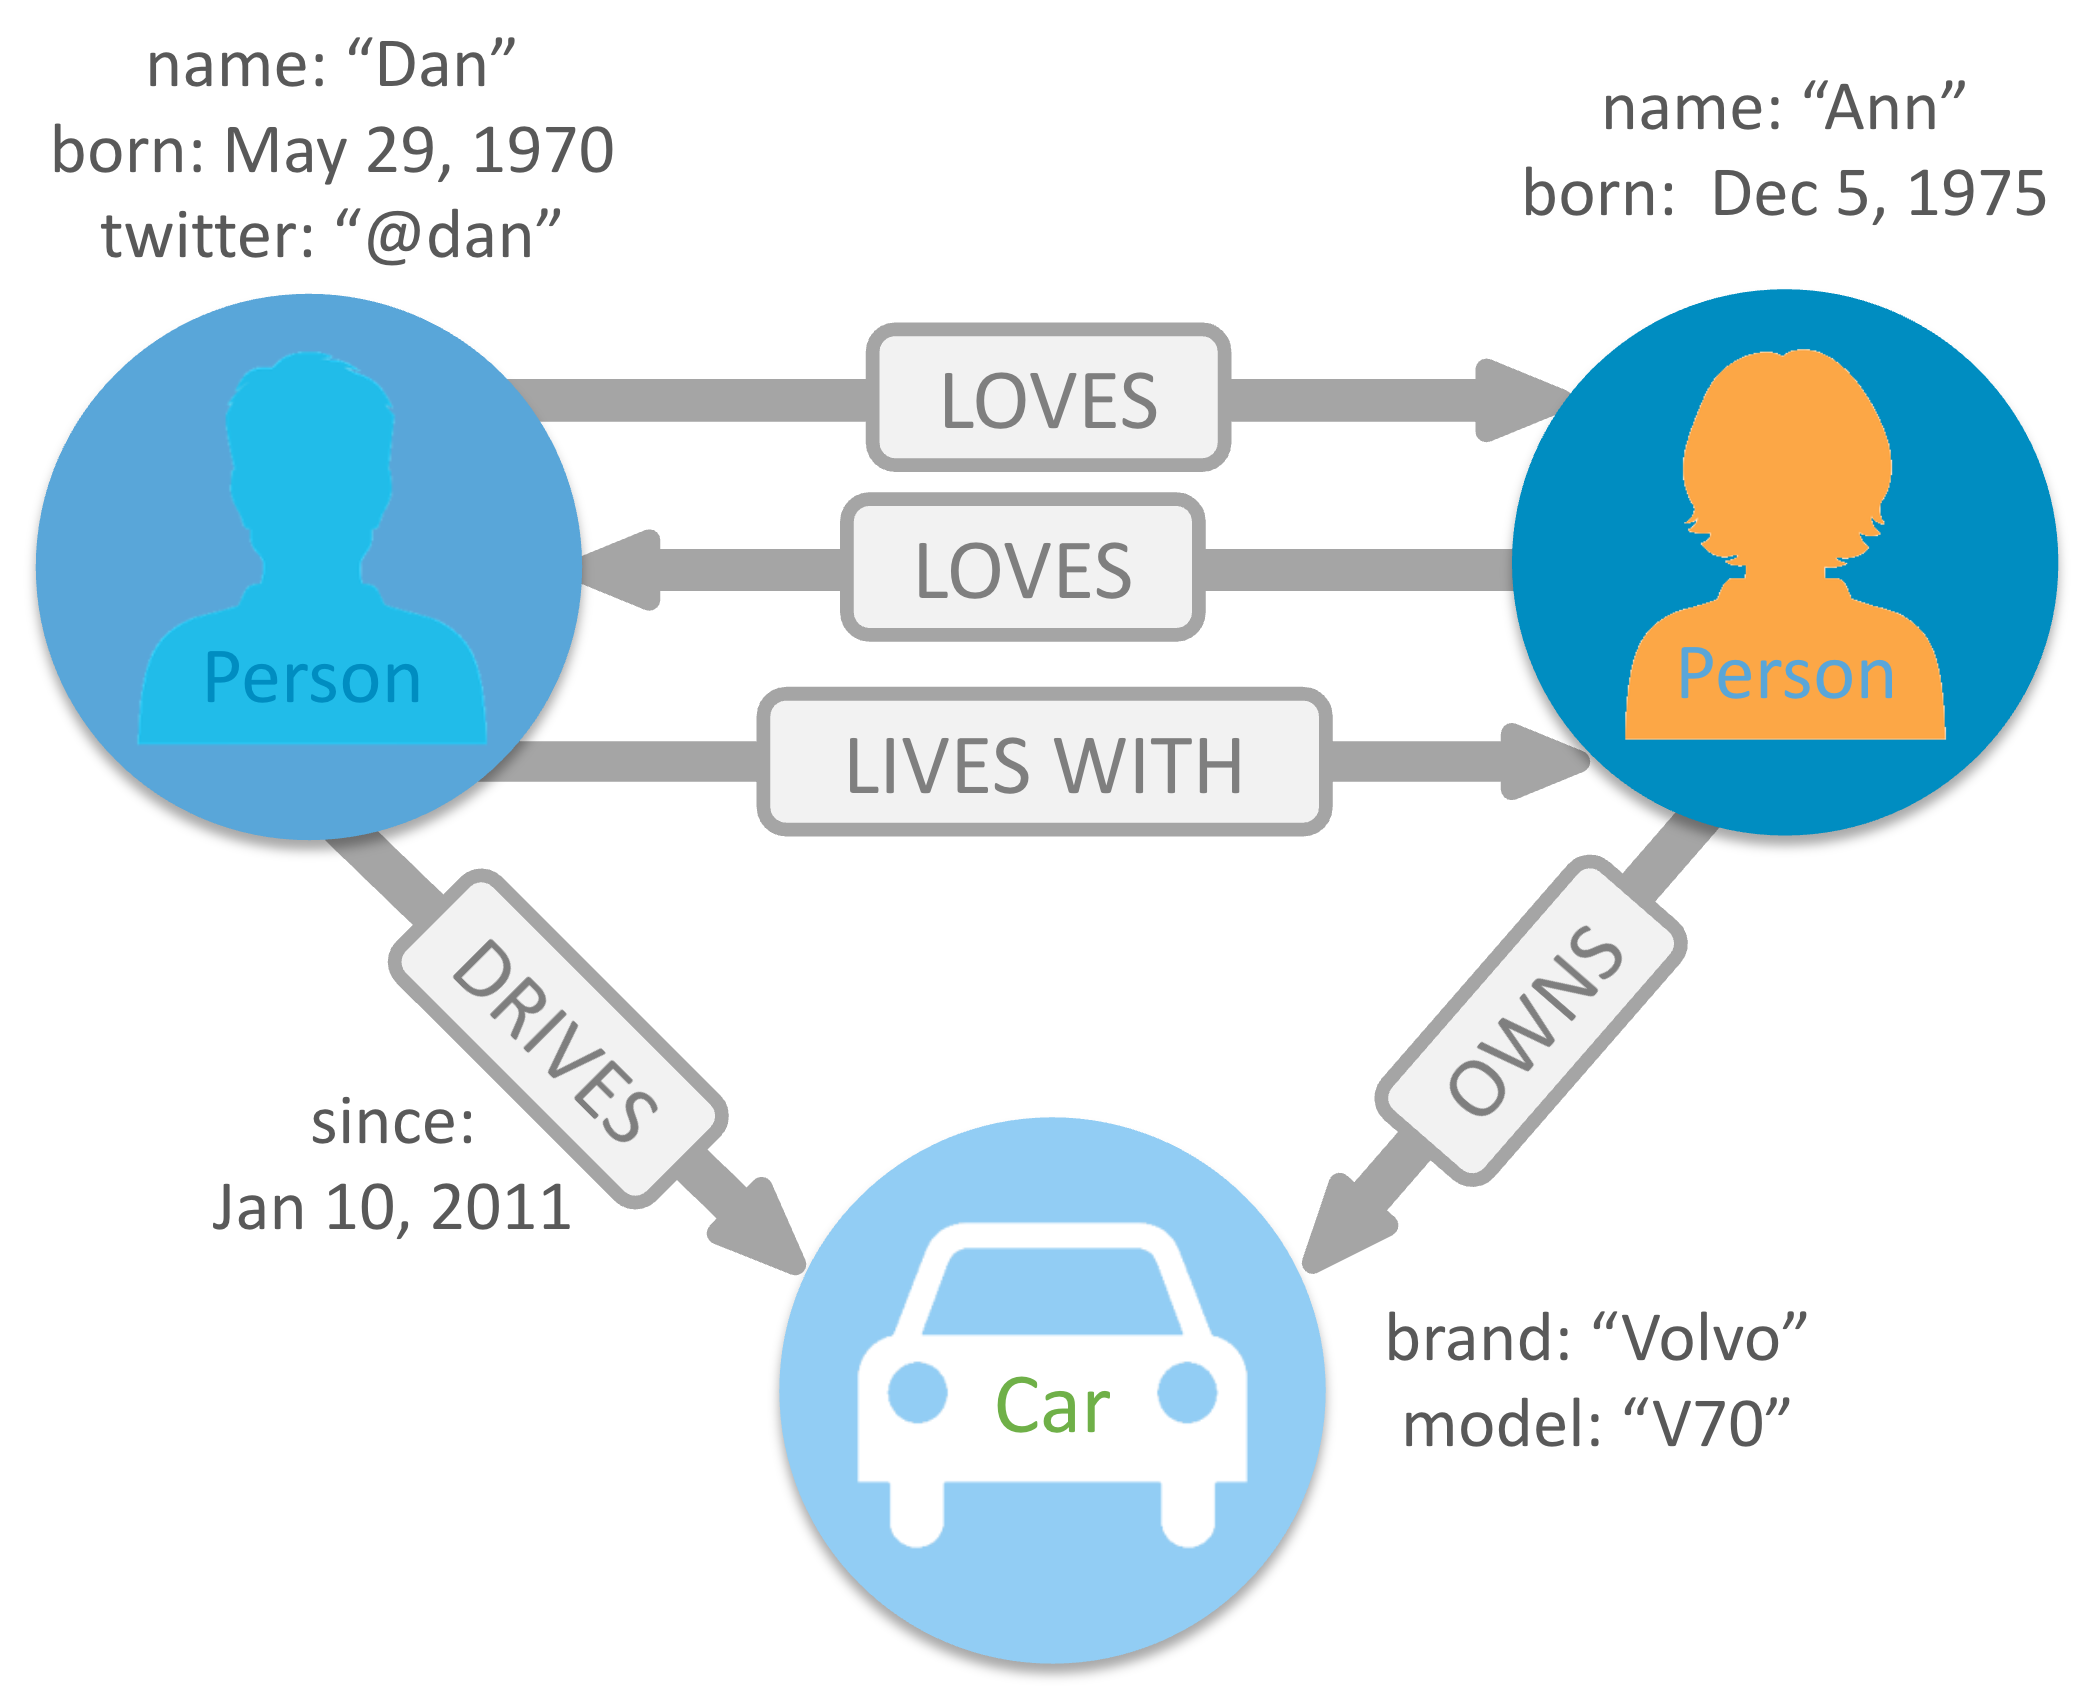
\includegraphics[width=8cm]{img/databaze/graph_db}
	\caption{Ukázka grafové databáze}
	\label{fig:db_img_graph}
	\end{figure}
\subsection{Dokumentová databáze}
Databáze dokumentů jsou typem NoSQL databáze a  jsou navržené pro ukládání, načítání a správu informací orientovaných na dokumenty. Dokumenty jsou obvykle uloženy ve formátu \gls{XML}, \gls{JSON}, \gls{BSON}. 
Typické příklady jsou: MongoDB, Amazon DocumentDB, Elasticsearch. Ukázku dokumentové databáze lze vidět na obrázku č. \ref{fig:db_img_document}.
	\begin{figure}[H]
	\centering
	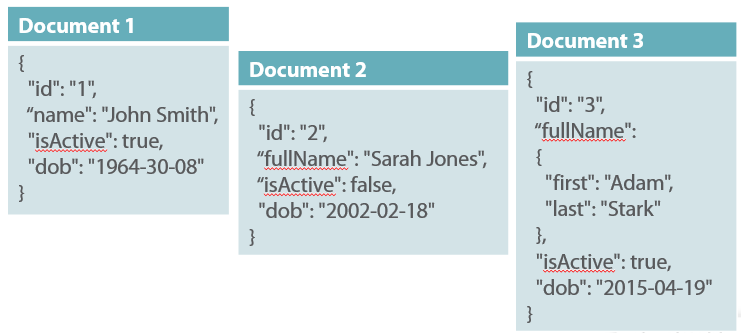
\includegraphics[width=11cm]{img/databaze/document_db}
	\caption{Ukázka dokumentově orientované databáze}
	\label{fig:db_img_document}
	\end{figure}

\section{Existující řešení}
Pro vybrané typy databáze existují mnoho databázových řešení, které lze zmínit. V této kapitole se budeme zabývat především těmi nejznámějšími pro daný typ databáze, a které jsou zdarma ke stažení a používání. Pro každý typ databáze byly vybrány maximálně dvě řešení.
\subsection{MySQL}
Relační
\subsection{PostgreSQL}
Relační
\subsection{ConceptBase}
OO
\subsection{LevelDB}
KeyValue
\subsection{Redis}
KeyValue
\subsection{MongoDB}
Document
\subsection{Elasticsearch}
Document
\subsection{Neo4j}
Graf
%%%%%%%%%%%%%%%%%%%%%%%%%%%%%%%%%%%%%%%%%%%%%%%%%%%%%%%%%%%%

%\chapter{Docker}
%\todo{todo}
%Popsat docker jako takový - kontejnery, image, docker compose, ...\newline
%\section{Kontejner vs Virtuální stroj}
\chapter{Návrh úložiště}

%This section provides a general overview of the state of today’s bibliographic
%databases and describes different types of bibliographical databases. First,
%we take a look at publication databases and show some examples of how they
%compare to each other. Next, we describe databases storing bibliographic
%information about patent data and provide some concrete examples of these
%data sources.

Zdroje (které ano, které ne + proč) + udělat stejnou tabulku jak v excelu + zmínit stránku ze který jsem čerpal informace (wipo.int)\todo{todo}\newline
Nezapomenout zmínit meze let, ve kterých se jednotlivé patenty z daných zemí nachází \todo{todo}

\section{Výběr patentů}
Při výběru patentů byly stanoveny tři podmínky, které museli být splněny:
\begin{itemize}
\item Dostupnost - patenty musí být dostupné z online stránek / databází bez poplatků.
\item Datum - patentová přihláška nebo publikace patentu musí být podána alespoň v roce 2000, všechny ostatní patenty budou vyfiltrovány.
\item Atributy - všechny patenty musí obsahovat povinné atributy (viz kapitola č. \ref{subsec:atributy}).
\end{itemize}

\subsection{Zdroje dat}
V dnešním světě existuje několik desítek až stovek patentových zdrojů dat, od webových vyhledávačů v databázi až po plný export databáze s patenty. Velké organizace, jako například \gls{EPO}, \gls{WIPO}, \gls{USPTO}, udržují jedny z největších patentových databází (desítky až stovky milionů patentů), ve kterých lze vyhledávat velké množství informací zdarma za použití webových vyhledávačů na dané stránce organizace. Lze zde najít všechny typy patentů (přihlášky, publikace), národní patenty i patenty registrované například u \gls{EPO}. V případě exportu databází, \gls{USPTO} poskytuje plný export svých databází veřejnosti pro libovolné používání, zcela zdarma. Využití těchto zdrojů dat by bylo určitě skvělé, ale tyto zdroje byly nedávno použity a rozebrány v jiné diplomové práci, proto je vhodné se spíše zaměřit na národní zdroje dat patentů.
\newline
\indent Národní databáze patentů dané země obsahuje všechny národní patenty, některé dokonce i patenty z jiných zemí registrovaných u \gls{EPO}. 
	\begin{table}[H]
	\centering
	\begin{tabular}{|>{\centering\arraybackslash}p{2.2cm}|>{\centering\arraybackslash}p{8cm}|>{\centering\arraybackslash}p{2cm}|} 
	\hline
	\textbf{Země}    & \textbf{Patentový úřad} & \textbf{Zkratka}                \\ 
	\hline
	Anglie & \href{https://www.gov.uk/topic/intellectual-property}{Intellectual Property Office}  & IPO         \\ 
	\hline
	Arménie & \href{https://www.aipa.am/hy/}{Intellectual Property Office}  & -         \\ 
	\hline
	Austrálie & \href{https://www.ipaustralia.gov.au/}{IP Australia}  & -         \\ 
	\hline
	Bělorusko & \href{https://www.ncip.by/}{National Center of Intellectual Property}  & NCIP         \\ 
	\hline
	Bulharsko & \href{https://www.bpo.bg/}{Patent Office of Republic of Bulgaria}  & -         \\ 
	\hline
	Česko & \href{https://upv.gov.cz/}{Industrial Property Office of the Czech Republic}  & -         \\ 
	\hline
	Čína & \href{https://www.cnipa.gov.cn/}{China National Intellectual Property Administration}  & CNIPA         \\ 
	\hline
	Dánsko & \href{https://www.dkpto.org/}{Danish Patent and Trademark Office}  & -         \\ 
	\hline
	Egypt & \href{http://www.egypo.gov.eg}{Egyptian Patent Office}  & -         \\ 
	\hline
	Estonsko & \href{https://www.epa.ee/et}{The Estonian Patent Office}  & -         \\ 
	\hline
	Filipíny & \href{http://www.ipophil.gov.ph/}{Intellectual Property Office of the Philippines}  & IPOPHL         \\ 
	\hline
	Finsko & \href{http://www.prh.fi/en/index.html}{Finnish Patent and Registration Office}  & PRH         \\ 
	\hline
	Francie & \href{http://www.inpi.fr/}{National Institute of Industrial Property}  & INPI         \\ 
	\hline
	Hong Kong & \href{https://www.ipd.gov.hk/index.htm}{Intellectual Property Department}  & -         \\ 
	\hline
	Chorvatsko & \href{https://www.dziv.hr/}{State Intellectual Property Office of the Republic of Croatia}  & SIPO         \\ 
	\hline
	Indie & \href{http://www.ipindia.nic.in/}{Office of the Controller General of Patents, Designs and Trade Marks}  & -         \\ 
	\hline
	Indonésie & \href{http://www.dgip.go.id/}{Directorate General of Intellectual Property}  & DGIP         \\ 
	\hline
	Irsko & \href{https://www.ipoi.gov.ie/en/}{Intellectual Property Office of Ireland}  & IPOI         \\ 
	\hline
	Island & \href{https://www.isipo.is/}{Icelandic Intellectual Property Office}  & ISIPO         \\ 
	\hline
	Israel & \href{https://www.gov.il/en/departments/ilpo}{The Israel Patent Office}  & ILPO         \\ 
	\hline
	Itálie & \href{https://uibm.mise.gov.it/index.php/it/}{Directorate General for the Protection of Industrial Property}  & -         \\ 
	\hline
	Japonsko & \href{https://www.jpo.go.jp/e/index.html}{Japan Patent Office}  & JPO         \\ 
	\hline
	Jižní Korea & \href{http://www.kipo.go.kr/}{Korean Intellectual Property Office}  & KIPO         \\ 
	\hline	
	Kanada & \href{https://www.ic.gc.ca/}{Canadian Intellectual Property Office}  & CIPO         \\ 
	\hline
	\end{tabular}
	\caption{Národní patentové úřady a jejich zkratky, část první}
	\label{tab:table_offices1}
	\end{table}

\newpage

	\begin{table}[H]
	\centering
	\begin{tabular}{|>{\centering\arraybackslash}p{2.2cm}|>{\centering\arraybackslash}p{8cm}|>{\centering\arraybackslash}p{2cm}|} 
	\hline
	\textbf{Země}    & \textbf{Patentový úřad} & \textbf{Zkratka}                \\ 
	\hline
	Kuba & \href{http://www.ocpi.cu}{Cuban Industrial Property Office}  & OCPI         \\ 
	\hline
	Litva & \href{http://vpb.lrv.lt/en/}{State Patent Bureau of the Republic of Lithuania}  & -         \\
	\hline
 	Lotyšsko & \href{https://www.lrpv.gov.lv/lv}{Patent Office of the Republic of Latvia}  & -         \\ 
	\hline
	Maďarsko & \href{http://www.hipo.gov.hu/}{Hungarian Intellectual Property Office}  & HIPO         \\ 
	\hline
	Malajsie & \href{http://www.myipo.gov.my/}{Intellectual Property Corporation of Malaysia}  & MyIPO         \\ 
	\hline
	Mexiko & \href{https://www.gob.mx/impi/en}{Instituto Mexicano De La Propiedad Industrial}  & IMPI         \\ 
	\hline
	Moldova & \href{http://www.agepi.gov.md/}{State Agency on Intellectual Property}  & AGEPI         \\ 
	\hline
	Německo & \href{http://www.dpma.de/}{German Patent and Trade Mark Office}  & DPMA         \\ 
	\hline
	Nizozemsko & \href{http://www.rvo.nl/octrooien}{Netherlands Patent Office}  & -         \\ 
	\hline
	Norsko & \href{https://www.patentstyret.no/en/}{Norwegian Industrial Property Office}  & NIPO         \\ 
	\hline
	Nový Zéland & \href{http://www.iponz.govt.nz/}{Intellectual Property Office of New Zealand}  & IPONZ         \\ 
	\hline
	Peru & \href{http://www.indecopi.gob.pe/}{National Institute for the Defense of Competition and Protection of Intellectual Property}  & INDECOPI         \\ 
	\hline
	Polsko & \href{https://uprp.gov.pl/pl}{Urząd Patentowy Rzeczypospolitej Polskiej}  & UPRP         \\ 
	\hline
	Portugalsko & \href{https://inpi.justica.gov.pt/}{Portuguese Institute of Industrial Property}  & -         \\ 
	\hline
	Rakousko & \href{http://www.patentamt.at/}{Austrian Patent Office}  & -         \\ 
	\hline
	Rumunsko & \href{http://www.osim.ro/}{State Office for Inventions and Trademarks}  & OSIM         \\ 
	\hline
	Rusko & \href{https://rospatent.gov.ru/}{Federal Service for Intellectual Property}  & Rospatent         \\ 
	\hline
	Řecko & \href{http://www.obi.gr/el/}{Hellenic Industrial Property Organization}  & HIPO         \\ 
	\hline
	Singapur & \href{http://www.ipos.gov.sg/}{Intellectual Property Office of Singapore}  & IPOS         \\ 
	\hline
	Slovensko & \href{https://www.indprop.gov.sk/}{Industrial Property Office of the Slovak Republic}  & -         \\ 
	\hline
	Slovinsko & \href{http://www.uil-sipo.si/}{Slovenian Intellectual Property Office}  & SIPO         \\ 
	\hline
	Srbsko & \href{http://www.zis.gov.rs/}{Intellectual Property Office of the Republic of Serbia}  & -         \\ 
	\hline
	Španělsko & \href{http://www.oepm.es/}{Spanish Patent and Trademark Office}  & OEPM         \\ 
	\hline
	Švédsko & \href{http://www.prv.se/}{Swedish Intellectual Property Office}  & PRV         \\ 
	\hline
	Švýcarsko & \href{https://www.ige.ch/}{Swiss Federal Institute of Intellectual Property}  & -         \\ 
	\hline
	Turecko & \href{http://www.turkpatent.gov.tr/}{Turkish Patent and Trademark Office}  & Turkpatent         \\ 
	\hline
	Ukrajina & \href{https://ukrpatent.org/en}{Ukrainian Intellectual Property Institute}  & Ukrpatent         \\ 
	\hline
	\end{tabular}
	\caption{Národní patentové úřady a jejich zkratky, část druhá}
	\label{tab:table_offices2}
	\end{table}

\newpage

\subsection{Atributy}\label{subsec:atributy}
\subsubsection{Povinné atributy}

	\begin{table}[H]
	\centering
	\begin{tabular}{|>{\centering\arraybackslash}p{2.2cm}|>{\centering\arraybackslash}p{2cm}|>{\centering\arraybackslash}p{3cm}|>{\centering\arraybackslash}p{2cm}|>{\centering\arraybackslash}p{2.5cm}|} 
	\hline
	\textbf{Země}    & \textbf{Název patentu} & \textbf{Rok přihlášky / publikace} & \textbf{Autor} & \textbf{ID patentu}                \\ 
	\hline
	Kanada & x & x & x & x \\
	\hline
	Česko & x & x & - & x \\
	\hline
	Litva & x & x & x & x \\
	\hline
	Portugalsko & x & x & x & x \\
	\hline
	Španělsko & x & x & x & x \\
	\hline
	Švédsko & - & x & - & x \\
	\hline
	Izrael & x & x & x & x \\
	\hline
	Itálie & x & x & x & x \\
	\hline
	Mexiko & x & x & x & x \\
	\hline
	Polsko & x & x & - & - \\
	\hline
	Anglie & x & x & x & x \\
	\hline
	Rusko & x & x & x & x \\
	\hline
	Peru & x & x & x & x \\
	\hline
	Francie & x & x & x & x \\
	\hline
	\end{tabular}
	\caption{Povinné atributy nacházející se v dostupných patentech}
	\label{tab:table_attributes_critical}
	\end{table}

\subsubsection{Nepovinné atributy}

	\begin{table}[H]
	\centering
	\begin{tabular}{|c|c|c|c|c|} 
	\hline
	\textbf{Země}    & \textbf{Abstrakt} & \textbf{Slovník} & \textbf{Reference} & \textbf{Žadatel} \\
	\hline
	Kanada & - & - & - & x \\
	\hline
	Česko & x & - & x & - \\
	\hline
	Litva & x & - & - & x \\
	\hline
	Portugalsko & x & - & - & x \\
	\hline
	Španělsko & x & - & - & x \\
	\hline
	Švédsko & x & - & - & - \\
	\hline
	Izrael & - & - & - & x \\
	\hline
	Itálie & - & - & - & x \\
	\hline
	Mexiko & x & - & - & x \\
	\hline
	Polsko & x & x & - & - \\
	\hline
	Anglie & - & - & - & - \\
	\hline
	Rusko & - & - & - & - \\
	\hline
	Peru & - & - & - & - \\
	\hline
	Francie & x & - & x & x \\
	\hline
	\end{tabular}
	\caption{Nepovinné atributy nacházející se v dostupných patentech, část první}
	\label{tab:table_attributes_notcrit1}
	\end{table}

	\begin{table}[H]
	\centering
	\begin{tabular}{|c|c|c|c|c|} 
	\hline
	\textbf{Země}    &  \textbf{Adresa} & \textbf{Rodina patentů} & \textbf{Obor} & \textbf{Fulltext} \\
	\hline
	Kanada & x & - & x & - \\
	\hline
	Česko & - & - & x & - \\
	\hline
	Litva & - & - & x & - \\
	\hline
	Portugalsko & - & - & x & - \\
	\hline
	Španělsko & x & - & x & x \\
	\hline
	Švédsko & - & - & x & x \\
	\hline
	Izrael & x & - & - & - \\
	\hline
	Itálie & - & - & - & - \\
	\hline
	Mexiko & - & - & x & - \\
	\hline
	Polsko & - & - & - & - \\
	\hline
	Anglie & - & - & x & - \\
	\hline
	Rusko & - & - & - & - \\
	\hline
	Peru & - & - & x & - \\
	\hline
	Francie & - & - & x & - \\
	\hline
	\end{tabular}
	\caption{Nepovinné atributy nacházející se v dostupných patentech, část druhá}
	\label{tab:table_attributes_notcrit2}
	\end{table}


\subsection{Závěr průzkumu}
Rovnou udělat kapitolu, ve který se aplikují všechny podmínky + se sepíše souhrn počtu patentů, z jakých zemí atp.


\section{Výběr databáze}
\todo{todo}
\subsection{Výběr typu databáze}
\subsection{Výběr z existujících řešení}
\subsection{Závěr průzkumu}
%%CHAPTER
\chapter{Návrh struktury}
% Co a jak bude propojeno ( + diagram)
% Import dat
%CHAPTER
\chapter{Implementace úložiště}
Výsledné řešení by mělo obsahovat dvě databáze, pomocí kterých bude možno vyhledávat patenty, ať už podle určitých atributů (ID, země, obor, a jiné), nebo pomocí full-textu. Vybrané databáze jsou uzpůsobeny pro ukládání velkého množství patentových dat, které byly staženy z národních zdrojů. 
\newline
\indent Import dat bude řešen pomocí vlastní aplikace, která bude filtrovat nevalidní patenty (neexistující povinné atributy, nevalidní \gls{XML} struktura, ...) a importovat validní patenty do databází. Pro MySQL databázi bude potřeba z patentu získat pouze specifické atributy.
\newline
\indent Výsledné řešení bude potřeba jednoduše nasadit na produkční server / počítač, aniž by bylo potřeba instalovat vícero aplikací. Řešení se postará o automatickou instalaci obou databází, jejich inicializaci (vytvoření tabulek, kolekcí, pohledů, ...) a zajistí propojení mezi databází \textbf{MongoDB} a full-textovým vyhledávačem \textbf{Elasticsearch}. S databázemi se zároveň nainstalují i aplikace pro jejich správu.

\section{Implementace databáze}
Pro databázi \textbf{MySQL} bylo navrženo a vytvořeno databázové schéma tak, aby bylo možno použít co nejvíce atributů při filtrování patentů pro statistiky. V \textbf{MongoDB} bude vytvořena databáze s jednou kolekcí, která bude obsahovat všechny vyfiltrované patenty.
\subsection{MongoDB}
Pro MongoDB byla použita jedna z nejnovějších verzí komunitní edice (verze 5.0.6). Programový systém \textbf{Mongo-express} (verze 0.54.0) bude použit jako nástroj pro spravování MongoDB databáze, ke kterému lze přistoupit pomocí webového prohlížeče.
\newline
\indent V databázovém schématu byla vytvořena databáze s názvem \textbf{patents}, která obsahuje pouze jednu kolekci s názvem \textbf{patents}. V této kolekci budou uloženy všechny vyfiltrované patenty ze všech zemí. Vzhledem k tomu, že MongoDB bude sloužit jen jako uložiště patentových dat, tak není potřeba vytvářet více kolekcí nebo databází. Jako další důvod pro zvolení pouze jedné kolekce je počet indexů v Elasticsearch, kdy byl použit pouze jeden index pro zaindexování všech dat. Důvod je takový, že chceme vždy prohledávat všechny patenty a ne jen jejich část, takže vícero indexů by akorát způsobovalo pomalejší zpracování dotazů pro vyhledávání.

\subsection{MySQL} \label{subsec:mysql_impl}
Pro MySQL byla použita verze komunitního serveru (verze 8.0.16). Programový systém \textbf{phpMyAdmin} (verze 5.1.3)  bude použit jako nástroj pro spravování MySQL databáze, ke kterému lze přistoupit pomocí webového prohlížeče. Lze použít i nástroj \textbf{MySQL Workbench} pro správu MySQL databáze, ale pro naše účely bohatě postačí \textbf{phpMyAdmin}.
\newline
\indent Schéma splňuje pouze druhou normální formu. Je to z toho důvodu, že tabulka \textbf{classification} obsahuje některé duplicitní hodnoty ve sloupcích. Duplicitu samozřejmě lze odstranit, ale zvýšilo by to složitost celého systému - \gls{SQL} dotazy by byly složitější a pomalejší v případě příkazu \textit{SELECT}, který by vyhledával data z několika tabulek, spojených příkazem \textit{JOIN}.
\newline

\noindent Databázové schéma pro MySQL lze vidět na obrázku č. \ref{fig:mysql_schema}.
\begin{figure}[H]
\centering
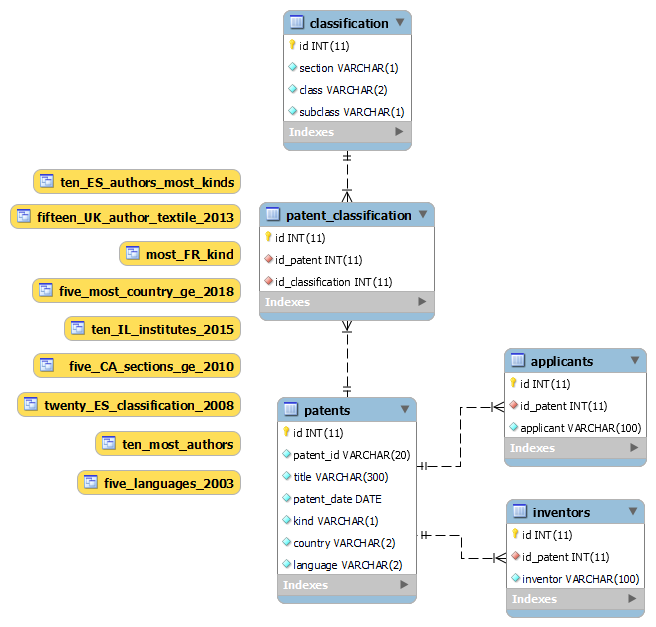
\includegraphics[width=12cm]{img/eer}
\caption{Schéma pro MySQL databázi.}
\label{fig:mysql_schema}
\end{figure}

\subsubsection{Tabulka patents}
Tabulka \textbf{patents} uchovává všechny národní patenty, které byly poskytnuty zdarma a obsahují všechny povinné atributy.

\subsubsection{Tabulka classification}
Tabulka \textbf{classification} slouží k uchovávání \gls{IPC} klasifikace daného patentu, konkrétně jeho sekci, třídu a podtřídu (skupina a podskupina vybrána nebyla, protože se vyskytovala v patentech jen ojediněle). 

\subsubsection{Tabulka patent\_classification}
Tabulka \textbf{patent\_classification} má kardinalitu \textit{M:N} a slouží jako propojení tabulky \textbf{patents} a tabulky \textbf{classification}. Jeden patent může mít více klasifikací (například se mohlo změnit označení v průběhu let, nebo patent pokrývá více oborů) a jedna klasifikace může být u více patentů.

\subsubsection{Tabulka inventors}
Tabulka \textbf{inventors} slouží k uchovávání jmen autorů patentů. Kardinalita mezi tabulkou \textbf{patents} a tabulkou \textbf{inventors} je \textit{1:N}, protože pro jeden patent může existovat více autorů.

\subsubsection{Tabulka applicants}
Tabulka \textbf{applicants} slouží k uchovávání jmen žadatelů patentů. Ačkoli existuje tabulka pro autory, tak může existovat scénář, ve kterém bude potřeba vyhledávat žadatele pro daný patent. Kardinalita mezi tabulkou \textbf{patents} a tabulkou \textbf{applicants} je \textit{1:N}, protože pro jeden patent může existovat více žadatelů.

\subsubsection{Pohledy}
Pohled je databázový objekt, který uživateli poskytuje data ve stejné podobě jako tabulka. Stručněji řečeno, je to struktura uchovávající \gls{SQL} dotaz, který se většinou dotazuje dané tabulky na specifická data.
\newline
\indent V databázi pro patenty bylo vytvořeno celkem devět pohledů, kdy každý z nich reprezentuje jeden scénář, který je použit při ověřování efektivního vytěžování (viz kapitola č. \ref{sec:efektivni_vytezovani_sql}).

\section{Nasazení úložiště}
Celý modul našeho úložiště čítá celkem 5 nástrojů - MySQL, MongoDB, Elasticsearch, phpMyAdmin a Mongo-express. Zároveň bude potřeba nastavit připojení mezi MongoDB a Elasticsearch tak, aby při přidání nového patentu do databáze byl následně zaindexován ve full-textovém vyhledávači. Pokud bychom měli po každém uživateli chtít instalaci všech těchto nástrojů a k tomu stahovat další nástroje pro vytvoření připojení mezi MongoDB a Elasticsearch, tak to zabere mnoho času a existuje zde velká pravděpodobnost že některé nástroje nebudou kompatibilní s aktuální verzí operačního systému. Z těchto důvodů byl zvolen software \textbf{Docker}, pomocí kterého se provede veškerá instalace a nastavení automaticky.

\subsection{Docker}
\textbf{Docker} je jeden z nejznámějších open-source nástrojů pro dodání aplikací v~balíčkách zvaných \textit{kontejner}. \textbf{Docker} využívá virtualizaci na úrovni operačního systému, čímž je výrazně snížena režie na rozdíl od klasických virtuálních strojů. Existují i jiné alternativy než docker, ale díky velké popularitě a fanouškovské základně byl vybrán právě docker.
\newline
\indent Definice a instalace aplikací je zajištěna pomocí nástroje \textbf{Docker compose}. Definice probíhá pomocí souboru s názvem \textit{docker-compose.yml} (viz obrázek č. \ref{fig:compose}), který využívá \gls{YAML} formát pro serializaci strukturovaných dat. V docker-compose.aml souboru pro tento modul je definováno celkem devět aplikací a dva nastavovací moduly. Data nejsou součástí inicializace kontejnerů, je potřeba je importovat dodatečně (dále viz kapitola \textbf{Uživatelská dokumentace}).
\begin{figure}[H]
\centering
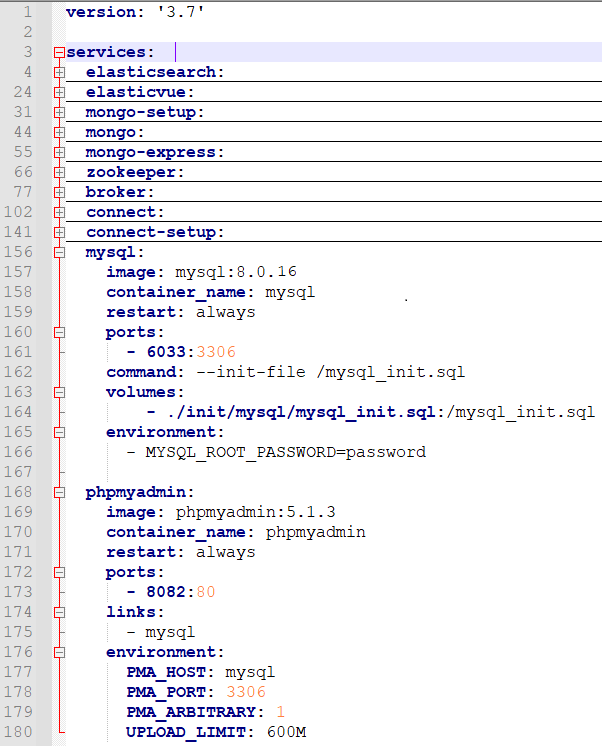
\includegraphics[width=11cm]{img/compose}
\caption{Ukázka souboru docker-compose.yml.}
\label{fig:compose}
\end{figure}

\subsubsection{Docker - Elasticsearch}
Pro Elasticsearch byly nadefinovány dvě aplikace:
\begin{itemize}
\item \textbf{elasticsearch} - Oficiální image full-textového vyhledávače Elasticsearch ve verzi 8.2.0. V nastavení byla vypnuto zabezpečení kvůli problémům se sadou replik v MongoDB.
\item \textbf{elasticvue} - Grafické uživatelské rozhraní pro Elasticsearch ve verzi 0.39.0, dostupné na localhostu na portu 8080.
\end{itemize}

\subsubsection{Docker - MongoDB}
Pro MongoDB byly nadefinovány dvě aplikace a jeden nastavovací modul:
\begin{itemize}
\item \textbf{mongo} - Oficiální image databáze MongoDB ve verzi 5.0.6. V databázi bylo nutné nastavit sadu replik, aby bylo možné vytvořit propojení mezi MongoDB a Elasticsearch.
\item \textbf{mongo-express} - Grafické uživatelské rozhraní pro MongoDB ve verzi 0.54.0, dostupné na localhostu na portu 8081.
\item \textbf{mongo-setup} - Nastavovací modul pro MongoDB, který po inicializaci databáze inicializuje sadu replik a následně vytvoří novou databázi a kolekci pro patenty.
\end{itemize}

\subsubsection{Docker - MongoDB a Elasticsearch konektor}
Pro konektor mezi MongoDB a Elasticsearch byly nadefinovány tři aplikace a jeden nastavovací modul:
\begin{itemize}
\item \textbf{broker} - Komunitní verze Apache Kafka od firmy Confluent ve verzi 6.1.0.
\item \textbf{zookeeper} - Nástroj pro Apache Kafka ve verzi 6.1.0, který funguje jako centralizovaná služba a slouží k údržbě jmenných a konfiguračních dat. Zároveň zajišťuje i flexibilní a robustní synchronizaci v rámci distribuovaných systémů.
\item \textbf{connect} - Nástroj pro Apache Kafka ve verzi 6.1.0, který má za úkol propojit externí systémy s Apache Kafka za pomoci konektorů.
\item \textbf{connect-setup} - Nastavovací modul pro Kafka connect, který po inicializaci Kafka connect vytvoří dva konektory:
	\begin{itemize}
	\item \textit{mongo-source-connector} - Konektor, který aktivně získává nová data z MongoDB a vkládá je do Kafka brokera.
	\item \textit{elasticsearch-sink-connector} - Konektor, který aktivně získává nová data z Kafka brokera a vkládá je do Elasticsearch.
	\end{itemize} 
\end{itemize}

\subsubsection{Docker - MySQL}
Pro MySQL byly nadefinovány dvě aplikace:
\begin{itemize}
\item \textbf{mysql} - Oficiální image databáze MySQL ve verzi 8.0.16. Při inicializaci databáze se vytvoří všechny tabulky i pohledy.
\item \textbf{phpmyadmin} - Grafické uživatelské rozhraní pro MySQL ve verzi 5.1.3, dostupné na localhostu na portu 8082. V nastavení byl navýšen limit pro import souborů na 600 MB z původních 2 MB.
\end{itemize}

\subsection{Inicializace MySQL}
Inicializace MySQL probíhá po vytvoření databáze v rámci docker kontejneru pro MySQL. Pro inicializaci byl vytvořen soubor \textbf{mysql\_init.sql}, který obsahuje příkazy pro vytvoření všech pěti tabulek (názvy tabulek, názvy sloupců, jejich omezení a klíče) a všech devíti pohledů.

\subsection{Inicializace MongoDB}
Inicializace MongoDB probíhá po vytvoření databáze v rámci docker kontejneru \textbf{mongo-setup}, protože MongoDB nemá žádnou možnost jak vložit inicializační soubor při startu kontejneru. Pro inicializaci byly vytvořeny dva soubory:
\begin{itemize}
\item \textbf{create\_mongo\_database.js} - Javascriptový soubor, který obsahuje příkazy pro vytvoření kolekce v databázi pro patenty.
\item \textbf{mongo\_init.sh} - Shell skript, který inicializuje sadu replik v databázi a následně spustí javascriptový soubor \textbf{create\_mongo\_database.js}.
\end{itemize}

\subsection{Propojení MongoDB a Elasticsearch}
Pro vytvoření spojení mezi MongoDB a Elasticsearch byly vyzkoušeny dva nástroje: \textbf{Mongo-connector} a \textbf{Apache Kafka}. 

\subsubsection{Mongo-connector}
Mongo-connector je obecný připojovací systém vyvinutý firmou MongoDB Inc. v roce 2012, který slouží pro integraci databáze MongoDB s jiným systémem, který podporuje \gls{CRUD} operace. Mongo-connector byl následně udržován pouze komunitně přibližně do roku 2018, kdy byla vydána poslední verze tohoto nástroje (verze 3.1.1).
\newline
\indent V původní verzi úložiště byl mongo-connector použit k propojení MongoDB ve verzi 5.0.6 a Elasticsearch ve verzi 7.17.0. Konektor pracoval rychle a bez problémů do té doby, než bylo potřeba použít novější verzi Elasticsearch (verze 8.x.x), kdy konektor nedokázal navázat žádné spojení a tím pádem nebylo možné využívat vyhledávač.
\newline
\indent Přechod na novější verzi Elasticsearch bylo potřeba z důvodu různých struktur patentů. Národní patentové úřady poskytují svá patentová data v~různých strukturách, které se mohou měnit v průběhu let, což byl i jeden z~důvodů pro výběr databáze MongoDB. V případě Elasticsearch je ale nutné, aby data měla stále stejnou strukturu, alespoň v rámci MongoDB kolekcí, protože Elasticsearch si data z kolekcí musí nejdříve zaindexovat pomocí mapperu a pak až v nich lze vyhledávat. V nejnovější verzi Elasticsearche (verze 8.x.x) je použit jiný způsob indexování souborů, takže data mohou mít libovolné struktury. Z tohoto důvodu byl mongo-connector zamítnut a musel být použit nový nástroj Apache Kafka.

\subsubsection{Apache Kafka}
Apache Kafka je distribuované úložiště událostí a platforma pro zpracování datových proudů (streamů). V diplomové práci byla použita Apache Kafka od firmy Confluent, která obsahuje dodatečné komunitní a komerční funkce navržené tak, aby vylepšily streamování operátorů i vývojářů v produkčním prostředí.
\newline
\indent Inicializace konektorů pro Apache Kafka probíhá v nastavovacím modulu \textbf{connect-setup}, ve kterém je stažen a nainstalován program \textbf{CURL}, který je využit shellovým skriptem \textbf{connect.sh}. Tento skript posílá dvě \gls{HTTP} POST metody na brokera (Apache Kafka), pomocí kterých se vytváří nové konektory. Na obrázku č. \ref{fig:sink} lze vidět data ve formátu JSON pro POST metodu, která vytvoří spojení z Apache Kafka do Elasticsearch, a na obrázku č. \ref{fig:source} lze vidět data pro vytvoření spojení z MongoDB do Apache Kafka.
\begin{figure}[H]
\centering
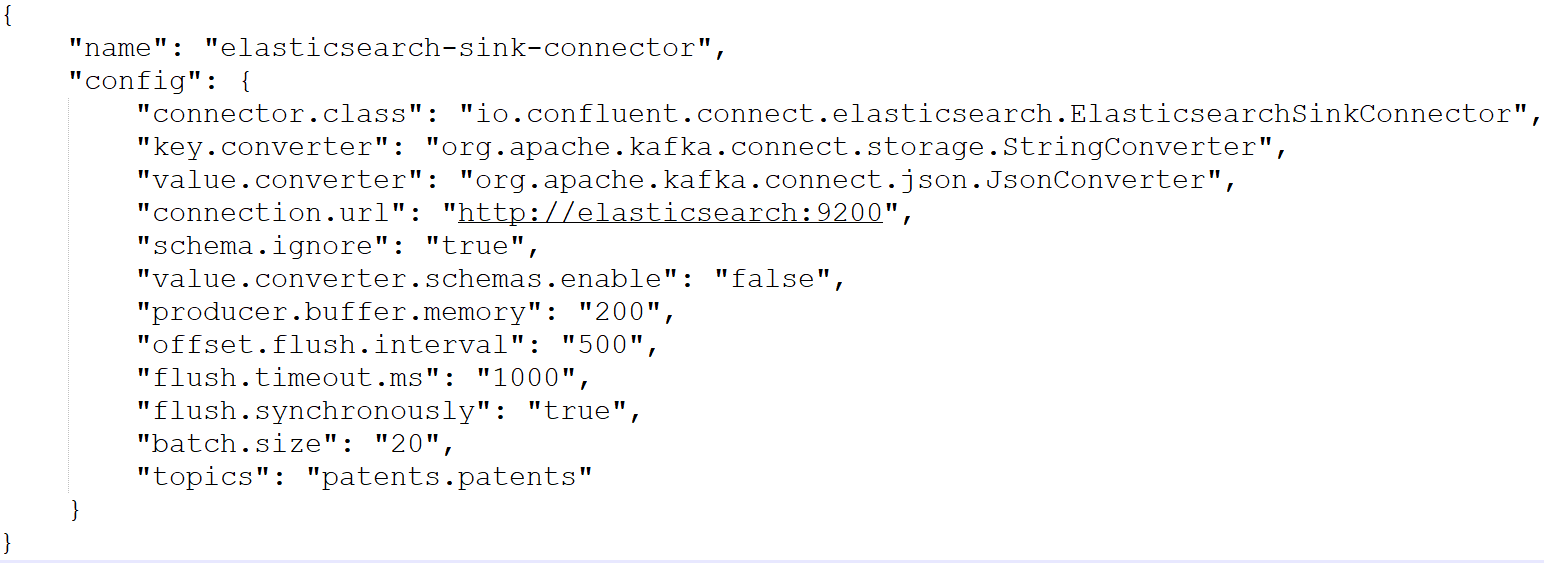
\includegraphics[width=15cm]{img/sink}
\caption{Data pro vytvoření konektoru z Apache Kafka do Elasticsearch.}
\label{fig:sink}
\end{figure}
\begin{figure}[H]
\centering
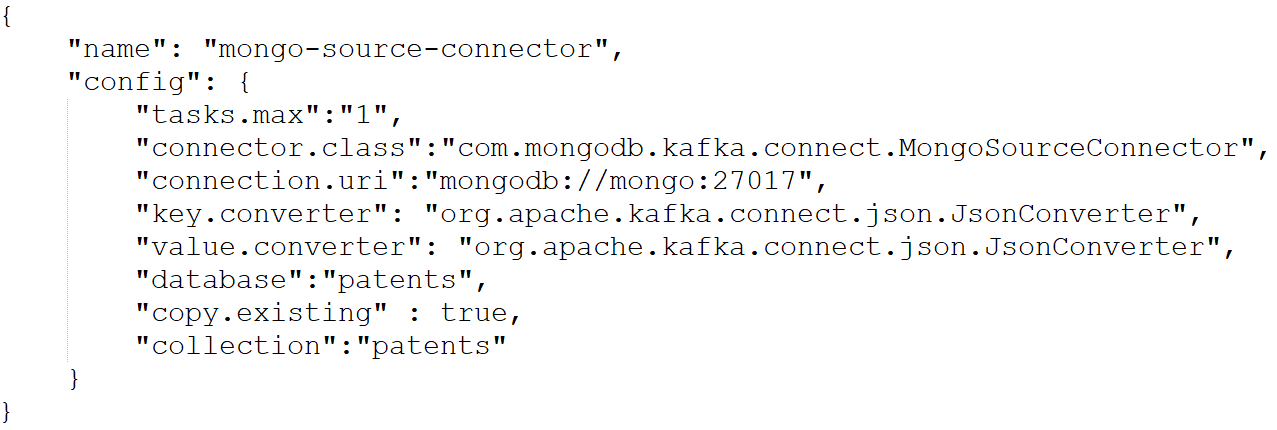
\includegraphics[width=14cm]{img/source}
\caption{Data pro vytvoření konektoru z MongoDB do Apache Kafka.}
\label{fig:source}
\end{figure}
%CHAPTER
\chapter{Rozšiřitelnost úložiště}
Zadání diplomové práce sice splněno bylo, ale v blízké budoucnosti mohou být požadavky na modul změněny. Jako příklad lze uvést podporu přidávání nových patentů do databází, zjištění autorů pro české patenty, automatické stahování dat z již ověřených patentových zdrojů. V této kapitole jsou popsány 3 možné návrhy na rozšíření modulu ohledně importu dat do již existujících databází.

\section{Přidávání nových patentů} \label{sec:new_patenty}
Cílem tohoto rožšíření by bylo automatické přidávání patentů z datových souborů jak do MySQL databáze, tak i do Mongo.

Rozšíření by se dalo realizovat jako aplikace ve vyšším programovacím jazyku (např. Java, C), kdy vstupem do aplikace by byl soubor v datovém formátu JSON/XML/CSV a jiné. Vstupní soubor by se následně:
\begin{itemize}
\item převedl na JSON řetězec (v případě že soubor není ve formátu JSON) a vložil do Mongo databáze
\item rozparsoval a extrahovali by se všechny atributy, které se ukládají v MySQL databázi (viz mysql kapitola \todo{TODO})
\end{itemize}

Jelikož je dost časté, že každý národní zdroj dat používá odlišnou strukturu patentu, tak bude potřeba aplikaci neustále upravovat (ať už v rámci přidávání nových zdrojů, nebo v případě změny struktury patentu u již podporovaných zdrojů).

Jako další velký problém lze zmínit extrakci atributů patentu ze souborů. Tím, že různé patentové soubory mají odlišnou strukturu, to znamená hloubku zanoření specifických elementů, jiné názvy elementů, tak bude obtížné naimplementovat řešení extrakce pro všechny soubory. Tento problém by se dal řešit tak, že se vytvoří soubory se slovníkama, které by obsahovali názvy elementů pro daný atribut. Slovníky by se následně použily při extrakci.

\section{Zjišťování autorů pro české patenty}
Český národní patentový úřad poskytuje data o českých patentech, které ale neobsahují autora ani instituci. Pro zjištění autora nebo instituce, která patent registrovala, je nutné použít oficiální vyhledávač. Cílem tohoto rozšíření by bylo vytvořit aplikaci ve vyšším programovacím jazyku, která se pro všechny české patenty bude snažit najít jejich autory za pomoci využití prohledávačů webů (web crawler). Postupů řešení může být mnoho:
\begin{itemize}
\item Zjišťování autorů by se provedlo pro všechny existující české patenty v databázi. Z MySQL databáze se zjistí všechny ID patentů pro české patenty, které se následně použijí jako vstup pro web crawler.
\item Zjišťování autorů by se provedlo pro patent/y uložené v souboru, kdy aplikace by pro všechny patenty v souboru zjistila autory a následně je dopsala do příslušnýho elementu patentu v daném souboru.
\item Stejný postup jako předchozí s tím rozdílem, že po zjištění autora se patent rovnou přidá do MySQL i Mongo databáze.
\end{itemize}

\section{Automatické stahování dat z ověřených zdrojů}
Cílem tohoto rozšíření by bylo automatické stahování dat (případně i jejich parsování) z ověřených zdrojů. Ověřené zdroje by byly uloženy například v XML souboru, kdy každý zdroj by měl tyto položky:
\begin{itemize}
\item \textbf{Název země}
\item \textbf{URL} - URL zdroje dat, na které lze stáhnout data.
\item \textbf{XPath} -  XPath výraz, pomocí kterého lze ze stránky vyfiltrovat a získat odkazy ke stažení dat\newline (např. \textit{/html/body//a[contains(@href,'example')]/@href})
\item \textbf{Poslední verze} - Název / číslo poslední stažené verze.
\end{itemize}
XML soubor by byl následně zpracován pomocí aplikace (např. Java, C\#), která by následně pro každý zdroj dat provedla následující kroky:
\begin{enumerate}
\item Získání seznamu odkazů na zdroje dat.
\item Stažení všech zdrojů dat, jejichž verze je větší než aktuálně uložená verze v XML.
\item V tomto bodě se dá naimplementovat cokoliv - např. lze uložená data extrahovat ze ZIP souborů, importovat patenty do databází (viz kapitola č. \ref{sec:new_patenty}), pouze notifikace o stažení několika nových souborů z daty a mnoho dalšího.
\item Aktualizace verze v XML souboru.
\end{enumerate}
Automatizace stahování dat by spočívala ve spouštění aplikace pro stahování dat v pravidelných intervalech (např. každé druhé úterý v 17:00). Jako příklad lze uvést použití pipeline na Jenkins serveru, který bude spouštět z lokálního uložiště spustitelnou aplikaci v daný čas (pomocí CRON). Po vykonání celého procesu může Jenkins poslat email o stavu posledního spuštění (zda se spuštění povedlo, kolik souborů byl schopen stáhnout pro jaké země, ...). Samozřejmě bohatě postačí i použití plánovače v OS.

\lstset{style=sqlstyle}

%CHAPTER
\chapter{Ověření efektivního vytěžování}
K ověření efektivního vytěžování bylo připraveno několik scénářů jak pro SQL, tak i pro Mongo + ElasticSearch.\newline
Napsat referenční stroj na kterém se testovalo - CPU, RAM, ...\todo{todo}
\section{Mongo + ElasticSearch}
\section{MySQL}
Pro MySQL bylo připraveno 10 scénářů, které testují všechny vytvořené tabulky v databázi. Každý scénář obsahuje textový popis, SQL příkaz, rychlost vykonání příkazu a ukázku výsledků.
\todo{vypsat počet hodnot v tabulkách}

\subsection{Scénář č.1}
\textbf{Textový popis}: Deset nejčastěji patentujících institucí v Izraeli v roce 2015.
\newline
\textbf{SQL}: 
\begin{lstlisting}[label = {lst:elements_a}]
select count(*), count(*) * 100.0 / ((select count(*) from inventors left outer join patents on inventors.id_patent = patents.id where YEAR(patents.patent_date) = 2015 and patents.patent_id like '%IL%') * 1.0) as percentage, inventors.inventor from inventors left outer join patents on inventors.id_patent = patents.id where YEAR(patents.patent_date) = 2015 and patents.patent_id like '%IL%' group by inventors.inventor order by count(*) desc, percentage desc LIMIT 10;
\end{lstlisting}
\textbf{Rychlost vykonání dotazu}: \todo{TODO}
\newline
\textbf{Výsledek dotazu}:\todo{TODO}
\begin{figure}[H]
\centering
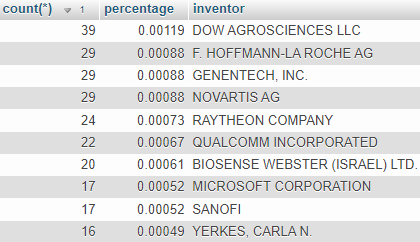
\includegraphics[width=7cm]{img/scenare/scenar_1}
\caption{Ukázka výsledku dotazu pro scénář č.1}
\label{fig:scenar1}
\end{figure}


\subsection{Scénář č.2}
\textbf{Textový popis}: Tři nejméně patentované obory v Kanadě od roku 2010.
\newline
\textbf{SQL}: 
\begin{lstlisting}[label = {lst:elements_a}]
select count(*), count(*) * 100.0 / ((select count(*) from classification left outer join patents on patents.id = classification.id_patent where YEAR(patents.patent_date) >= 2010 and patents.patent_id like '%CA%') * 1.0) as percentage, classification.section from classification left outer join patents on patents.id = classification.id_patent where YEAR(patents.patent_date) >= 2010 and patents.patent_id like '%CA%' group by classification.section order by count(*) asc, percentage asc LIMIT 5;
\end{lstlisting}
\textbf{Rychlost vykonání dotazu}: \todo{TODO}
\newline
\textbf{Výsledek dotazu}:\todo{TODO}
\begin{figure}[H]
\centering
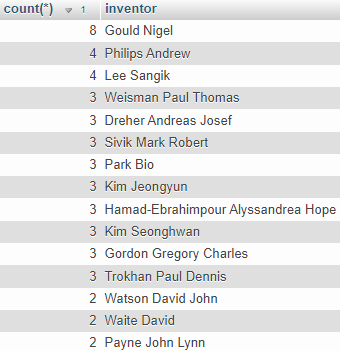
\includegraphics[width=6cm]{img/scenare/scenar_9}
\caption{Ukázka výsledku dotazu pro scénář č.2}
\label{fig:scenar2}
\end{figure}

\subsection{Scénář č.3}
\textbf{Textový popis}: Dvacet nejčastějších klasifikací patentů za rok 2008 ve Španělsku.
\newline
\textbf{SQL}:
\begin{lstlisting}[label = {lst:elements_a}]
select count(*), count(*) * 100.0 / ((select count(*) from classification left outer join patents on patents.id = classification.id_patent where YEAR(patents.patent_date) = 2008 and patents.patent_id LIKE '%ES%') * 1.0) as percentage, classification.section, classification.class, classification.subclass from classification left outer join patents on patents.id = classification.id_patent where YEAR(patents.patent_date) = 2008 and patents.patent_id LIKE '%ES%' group by classification.section, classification.class, classification.subclass order by count(*) desc, percentage desc LIMIT 20;
\end{lstlisting}
\textbf{Rychlost vykonání dotazu}: \todo{TODO}
\newline
\textbf{Výsledek dotazu}:\todo{TODO}
\begin{figure}[H]
\centering
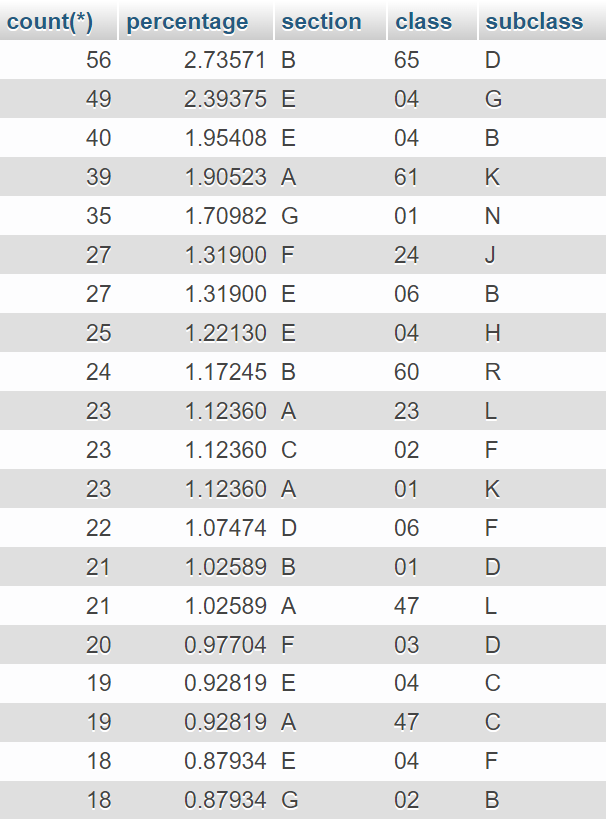
\includegraphics[width=7cm]{img/scenare/scenar_3}
\caption{Ukázka výsledku dotazu pro scénář č.3}
\label{fig:scenar3}
\end{figure}

\subsection{Scénář č.4} 
\textbf{Textový popis}: Deset autorů s největším počtem patentů ze všech zemí.
\newline
\textbf{SQL}: \todo{divnej dotaz}
\begin{lstlisting}[label = {lst:elements_a}]
select count(*), count(*) * 100.0 / ((select count(*) from inventors) * 1.0) as percentage, inventors.inventor from inventors left outer join patents on patents.id = inventors.id_patent group by inventors.inventor order by count(*) desc, percentage desc LIMIT 10;
\end{lstlisting}
\textbf{Rychlost vykonání dotazu}: \todo{TODO}
\newline
\textbf{Výsledek dotazu}:\todo{TODO}
\begin{figure}[H]
\centering
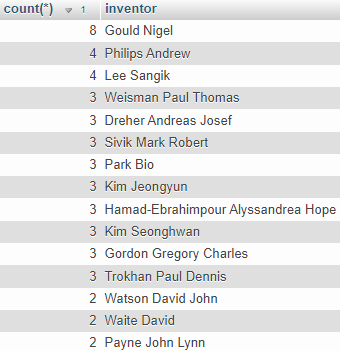
\includegraphics[width=6cm]{img/scenare/scenar_9}
\caption{Ukázka výsledku dotazu pro scénář č.4}
\label{fig:scenar4}
\end{figure}

\subsection{Scénář č.5}
\textbf{Textový popis}: Pět nejméně používaných jazyků pro patenty za rok 2003.
\newline
\textbf{SQL}: 
\begin{lstlisting}[label = {lst:elements_a}]
select count(*), count(*) * 100.0 / ((select count(*) from patents where patents.language not like '%-%') * 1.0) as percentage, patents.language from patents where patents.language not like '%-%' group by patents.language order by count(*) asc, percentage asc LIMIT 5;
\end{lstlisting}
\textbf{Rychlost vykonání dotazu}: \todo{TODO}
\newline
\textbf{Výsledek dotazu}:\todo{TODO}
\begin{figure}[H]
\centering
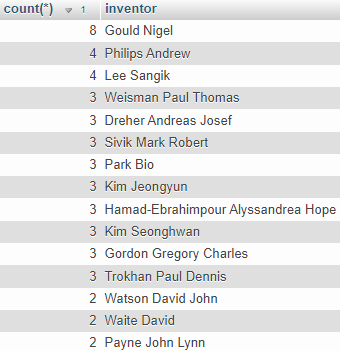
\includegraphics[width=6cm]{img/scenare/scenar_9}
\caption{Ukázka výsledku dotazu pro scénář č.5}
\label{fig:scenar5}
\end{figure}

\subsection{Scénář č.6}
\textbf{Textový popis}: Deset Institucí / autorů s patenty pokrývající největší množství oborů.
\newline
\textbf{SQL}: 
\begin{lstlisting}[label = {lst:elements_a}]
select count(distinct classification.section), count(*) * 100.0 / ((select count(*) from inventors left outer join classification on classification.id_patent = inventors.id_patent where section is not null) * 1.0) as percentage, inventors.inventor from inventors left outer join classification on classification.id_patent = inventors.id_patent where section is not null group by inventors.inventor order by count(distinct classification.section) desc, percentage desc LIMIT 10;
\end{lstlisting}
\textbf{Rychlost vykonání dotazu}: \todo{TODO}
\newline
\textbf{Výsledek dotazu}:\todo{TODO}
\begin{figure}[H]
\centering
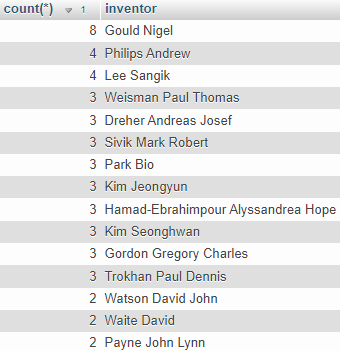
\includegraphics[width=6cm]{img/scenare/scenar_9}
\caption{Ukázka výsledku dotazu pro scénář č.6}
\label{fig:scenar6}
\end{figure}

\subsection{Scénář č.7}
\textbf{Textový popis}: Pět zemí s nejvíce patenty od roku 2018.
\newline
\textbf{SQL}: 
\begin{lstlisting}[label = {lst:elements_a}]
select count(*), count(*) * 100.0 / ((select count(*) from patents where YEAR(patents.patent_date) >= 2018) * 1.0) as percentage, patents.country from patents where YEAR(patents.patent_date) >= 2018 group by patents.country order by count(*) desc, percentage desc LIMIT 5;
\end{lstlisting}
\textbf{Rychlost vykonání dotazu}: \todo{TODO}
\newline
\textbf{Výsledek dotazu}:\todo{TODO}
\begin{figure}[H]
\centering
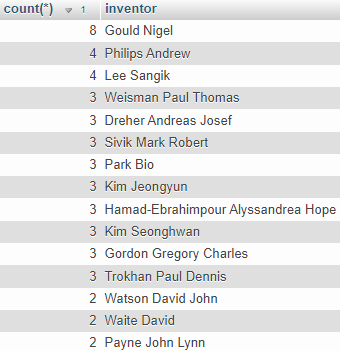
\includegraphics[width=6cm]{img/scenare/scenar_9}
\caption{Ukázka výsledku dotazu pro scénář č.7}
\label{fig:scenar7}
\end{figure}

\subsection{Scénář č.8}
\textbf{Textový popis}: Nejvíce používaný jazyk pro patenty ve Francii.
\newline
\textbf{SQL}: 
\begin{lstlisting}[label = {lst:elements_a}]
select count(*), count(*) * 100.0 / ((select count(*) from patents where patents.patent_id like '%FR%') * 1.0) as percentage, patents.language from patents where patents.patent_id like '%FR%' group by patents.language order by count(*) desc, percentage desc;
\end{lstlisting}
\textbf{Rychlost vykonání dotazu}: \todo{TODO}
\newline
\textbf{Výsledek dotazu}:\todo{TODO}
\begin{figure}[H]
\centering
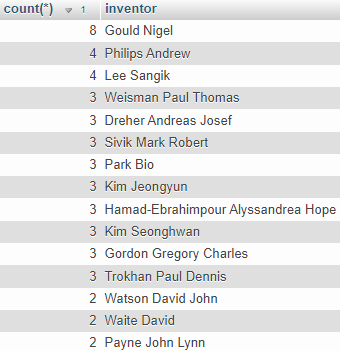
\includegraphics[width=6cm]{img/scenare/scenar_9}
\caption{Ukázka výsledku dotazu pro scénář č.8}
\label{fig:scenar8}
\end{figure}

\subsection{Scénář č.9}
\textbf{Textový popis}: Patnáct nejčastěji patentujících institucí / autorů v Anglii v textilním oboru za rok 2013.
\newline
\textbf{SQL}: 
\begin{lstlisting}[label = {lst:elements_a}]
select count(*), count(*) * 100.0 / ((select count(*) from inventors left outer join patents on patents.id = inventors.id_patent left outer join classification on classification.id_patent = patents.id where classification.section like '%D%' and patents.patent_id like '%GB%' and YEAR(patents.patent_date) = 2013) * 1.0) as percentage, inventors.inventor from inventors left outer join patents on patents.id = inventors.id_patent left outer join classification on classification.id_patent = patents.id where classification.section like '%D%' and patents.patent_id like '%GB%' and YEAR(patents.patent_date) = 2013 group by inventors.inventor order by count(*) desc, percentage desc LIMIT 15;
\end{lstlisting}
\textbf{Rychlost vykonání dotazu}: \todo{TODO}
\newline
\textbf{Výsledek dotazu}:\todo{TODO}
\begin{figure}[H]
\centering
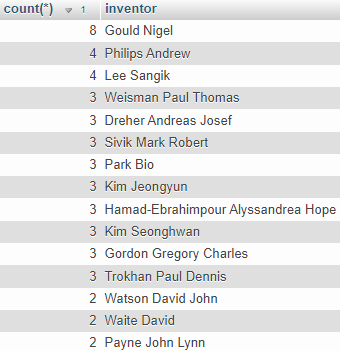
\includegraphics[width=7cm]{img/scenare/scenar_9}
\caption{Ukázka výsledku dotazu pro scénář č.9}
\label{fig:scenar9}
\end{figure}
%CHAPTER
\chapter{Závěr}
V rámci této práce se autor seznámil s dostupnými zdroji dat o patentech. Celosvětové patentové instituce nebyly prostudovány z důvodu již existující diplomové práce \cite{BARATTA2019thesis}, která byla zaměřená právě na tyto celosvětové instituce. Tato diplomová práce rozšiřuje původní diplomovou práci ve směru národních patentujících institucí a jejich dat.
\newline
\indent Celkem bylo prostudováno 51 národních patentových institucí z celého světa. U institucí byla zkoumána hlavně dostupnost patentových dat (zda patentová instituce poskytuje svá data ke stažení zdarma nebo za peníze) a validita dat. Data byla vyhodnocena jako validní tehdy, když obsahovali všechny povinné atributy, kterými jsou: ID patentu, titulek patentu, datum přihlášení a existující autor. Z 51 národních patentových institucí splňovalo tyto dvě podmínky pouze 10 institucí, které poskytly necelé dva miliony validních záznamů o patentových dat.
\newline
\indent Vzhledem k získaným datům z patentových institucí byly prozkoumány možné typy databází, které by umožňovali jejich efektivní vytěžování. Při průzkumu bylo porovnáváno pouze šest nejznámějších typů databází, které by mohli ukládat patentová data. Z šesti typů dat byly nakonec vybrány dva typy databází, každý pro jiný účel. První typ, relační databáze, poslouží k~rychlému získávání statistik o patentech. Druhý typ, databáze dokumentů, poslouží k ukládání celých souborů s patentovými daty. Jako existující řešení pro relační databázi bylo vybráno MySQL, pro databázi dokumentů zase MongoDB, které se pomocí Apache Kafka propojilo s full-textovým vyhledávačem Elasticsearch. Vzhledem ke vstupním datům, která jsou uložena v několika různých strukturách, bylo dokázáno, že kombinace relační a dokumentové databáze může být velice dobré řešení. Udržování obou databází může být časově a kapacitně náročnější, ale rychlost a efektivita vyhledávání je větší než v případě použití pouze jedné databáze.
\newline
\indent Zadání práce bylo splněno ve všech bodech. Zvolená databázová řešení umožňují efektivní vytěžování patentových dat pomocí full-textového vyhledávače Elasticsearch v případě MongoDB, a pomocí \gls{SQL} dotazů v MySQL pro získávání statistik. Efektivní vytěžování bylo otestováno na třech scénářích pro MongoDB, a devíti scénářích pro MySQL. Instalace všech nástrojů a databází se provádí pomocí Dockeru.

%%%%%%%%%%%%%%%%%%%%%%%%%%%%%%%%%%%%%%%%%%%%%%%%%%%%%%%%%%
%
% Zkratky
%
%%%%%%%%%%%%%%%%%%%%%%%%%%%%%%%%%%%%%%%%%%%%%%%%%%%%%%%%%%

\printglossary[type=\acronymtype,title={Zkratky}]
 
%%%%%%%%%%%%%%%%%%%%%%%%%%%%%%%%%%%%%%%%%%%%%%%%%%%%%%%%%%
%
% LITERATURA
%
%%%%%%%%%%%%%%%%%%%%%%%%%%%%%%%%%%%%%%%%%%%%%%%%%%%%%%%%%%

\bibliographystyle{csplainnatkiv}
{\raggedright\small
\bibliography{literature/literatura}
}

%%%%%%%%%%%%%%%%%%%%%%%%%%%%%%%%%%%%%%%%%%%%%%%%%%%%%%%%%%
%
% PŘÍLOHA
%
%%%%%%%%%%%%%%%%%%%%%%%%%%%%%%%%%%%%%%%%%%%%%%%%%%%%%%%%%%
\setcounter{chapter}{0}
\renewcommand{\thechapter}{\Alph{chapter}}

%CHAPTER
\chapter{Uživatelská dokumentace}
% Postup instalace + i obrázky - po instalaci všech image obrázek z dockeru, po inicializaci MySQL v PHPMyAdmin, po inicializaci MongoDB v Mongo-express a Elasticsearch v Elasticvue
%CHAPTER
\chapter{Vzhled PDF formuláře}\label{chap:vysledny_vzhled_formulare}
\begin{center}
\begin{minipage}[b]{0.95\textwidth}
	%\framebox{
		\includepdf[pages=1,pagecommand={},frame,width=0.95\textwidth]{pdf/vysledny_vzhled.pdf}
	%}
\end{minipage}
\end{center}
\newpage
\begin{center}
\begin{minipage}[b]{0.95\textwidth}
	%\framebox{
		\includepdf[pages=2,pagecommand={},frame,width=0.95\textwidth]{pdf/vysledny_vzhled.pdf}
	%}
\end{minipage}
\end{center}

%%%%%%%%%%%%%%%%%%%%%%%%%%%%%%%%%%%%%%%%%%%%%%%%%%%%%%%%%%
%
% KONEC TEXTU PRÁCE
%
%%%%%%%%%%%%%%%%%%%%%%%%%%%%%%%%%%%%%%%%%%%%%%%%%%%%%%%%%%
\end{document}
